\chapter{Methods}
To be able to evaluate the performance of using Erlang to communicate in a WSN two prototypes need to be developed. From these prototypes data is going to be collected. After the data is collected, the data is going to be analysed to show when Erlang can be an alternative to a low-level language in a WSN. 

\section{Setup}
The prototypes that has been develop is as mentioned in previous sections are prototypes of a  video-based sensor network. A basic idea of how the network has been constructed can be seen in Figure~\ref{fig:setup}. This figure shows how the network is looking like for the case of the experiments preformed in this thesis, but the network design of the final product must not necessary look like this. 

\begin{figure}[H]
\centering
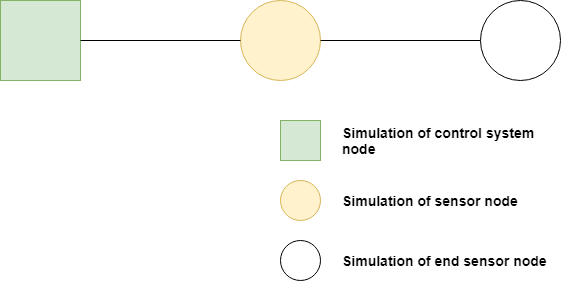
\includegraphics[scale=0.6]{figure/setup.png}
\caption{The idea of the video-based sensor network in the case of this experiment.}
\label{fig:setup}
\end{figure}

There can be arbitrarily many sensor nodes in the network but there is no need for the network to be bigger than the one shown in Figure~\ref{fig:setup} for the investigation in this thesis. This is because the sensor that has been investigated is a sensor that both receive data from another sensor and sends data to another device and that is fulfilled with the current network setup. This means that all measurements presented in this thesis is from the node in the middle of Figure~\ref{fig:setup}. 

The hardware to simulate the sensor that has been investigated is a Freescale i.MX 6Quad SABRE Development Board with a 1GHz ARM Cortex A9 core and 1 GB DDR3 SDRAM with up to 533 MHz memory \citep{nxp2012board}. The investigation does not focus on the other devices in the network and therefor there is no specific requirements on these devices except that they need to have sufficient hardware capacity to not slow down the execution of the prototypes. Because of this the devices in this case was simulated by using two PC computers.  

To achieve communication between the devices in the network ZigBee was used. The i.MX 6 board does not have built in support for the IEEE 802.15.4 standard so therefore some module was needed to add support to the i.MX 6 board.  

The modules that was used for the experiments in this thesis was the modules from the XBee ZigBee Mesh Kit (XKB2-Z7T-WZM). This kit consists of three Xbee ZigBee modules and three Grove development boards. By mounting the Xbee ZigBee modules in the Grove development boards and connecting the boards with a USB to the processing unit, it is possible for the processing unit to communicate with the connected Xbee ZigBee module. 
 
There are many alternatives for operating system but because the company uses a basic Debian distribution in their other products and want to continue using it. It is this operating system that is going to be used for the sensor that is going to be investigated.

\section{Prototypes}
To be able to evaluate if Erlang is an alternative to a low-level language in developing the communication between sensors in a WSN, two prototypes was implemented. The first prototype was developed by using the C++ language and the other was developed with the Erlang language. 

The first step in the prototypes’ development process was to decide on a design. In this case the design is how the sensors in the network shall communicate. For example, shall a sensor ask for its child sensor’s data or shall the child sensor pass data to its parent without being asked for it.

After this first decision was made the approach to developing the prototypes was the same iterative approach for both, where each step was a small step towards completing the communication parts that was needed to evaluate if Erlang can manage the communication in the final product of the company. The choice of this iterative approach was to give the possibility of catching problems early and to only implement as much of the communication code that was needed to carry out the evaluation.

\subsection{C++ prototype}
The structure of the C++ prototype is divided in three processes. The task of the first process, the Writer process, is to receive the data output from the other two processes and sending it to the ZigBee module for transmission to the correct recipient. The second process is the Datagen process that simulate the generation of data and the last process, the Reader process, is responsible for collecting incoming data from another device in the network.

The communication between a process and a ZigBee module is done by first opening a serial port and after that the communication is simply done by reading and writing to this port. The settings that the port needs to be configured with can be found in the implementations of the C++ prototype found in Appendix~\ref{appendix:cpp_prototype} Section~\ref{secA:serial_port}.

For the Datagen and Reader process to communicate data to the Writer process dbus was used. Dbus provides interprocess communication in the form of a server-client behaviour. The Writer process implements functionality that listens to incoming messages from the Datagen and Reader process. The implementation of this can be seen in Appendix~\ref{appendix:cpp_prototype}.

The last consideration in the development of the C++ prototype was about fault-tolerance. If one of the processes would crash, it should be restarted automatically. To solve this systemd was used. By turning the processes into services systemd can restart them after the provided specifications that can be seen in Appendix~\ref{appendix:cpp_prototype} Section~\ref{secA:systemd}. 

\subsection{Erlang prototype}
According to the Erlang homepage it is very hard to implement a new driver for the distribution carrier and therefore the choice for the connection between Erlang and a ZigBee module was for this thesis to implement a port or a port driver \citep{ericsson_ab_2019}. 

Ports, port drivers, C nodes and Native Implemented Functions (NIFs) is different methods that is provided by Erlang for and Erlang application to run C code. The difference between these methods are in how they are loaded. For example, NIFS are dynamically linked into the emulator process and port drivers are a shared library and these methods to load the C code would cause the emulator to crash if the C code terminates. A representation of the loading differences between a port and a port drivers can be seen in Figure~\ref{fig:erlang_run_ccode} \citep{ericsson_ab_2019}. 

\begin{figure}[H]
\centering
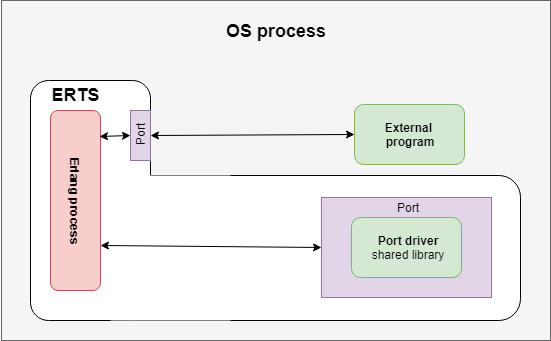
\includegraphics[scale=0.77]{figure/port_portdriver.png}
\caption{Figure showing the difference between a port and a port driver.}
\label{fig:erlang_run_ccode}
\end{figure}

As mentioned if a port driver crashes the emulator also crashes. Therefor the choice was made to use a port. For the implementation of the port much of the code from the C++ prototype could be reused and the full implementation can be seen in Appendix~\ref{appendix:erlang_prototype} Section~\ref{secB:port}.

The Erlang prototype has a similar structure as the C++ prototype, a Writer, Reader and Datagen process. A difference is that it instead of using systemd for restarting something that has crashed, the built-in supervisor behaviour of Erlang is used instead. By building a supervisor tree it is possible to specify how the restart procedure shall be performed in the event of a crash. A model of the supervisor tree is shown in Figure~\ref{fig:erlang_structure_prototype} and the full implementation of the prototype can be seen in Appendix~\ref{appendix:erlang_prototype}.

\begin{figure}[H]
\centering
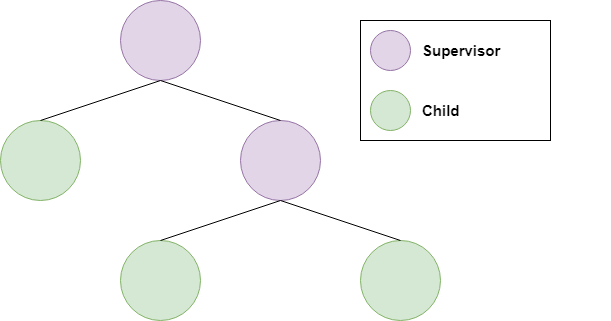
\includegraphics[scale=0.65]{figure/erlang_structure_prototype.png}
\caption{The structure of the Erlang prototype.}
\label{fig:erlang_structure_prototype}
\end{figure}

The specified restart procedure for the root supervisor is that if one of the processes crashes all process is restarted. This choice was made for two reasons. First, if the writer process has crashed the work done by the reader and datagen process is wasted because there is no recipient for the data they sends out. Secondly, to send massages to the writer process the other processes need to know the pid of the process. This knowledge is achieved by the writer process registering its pid to an atom, which is an Erlang literal. If a process then try to use this atom to send a message when the writer has crashed it also crashes. The second supervisor only supervises children that has no dependant processes. Therefore, the restart strategy is to only restart the child that has crashed. 

\section{Data collection}\label{sec:data_collection}
Data was collected from the two prototypes for the purpose of evaluating the performance of using Erlang in a WSN. The collected data was in all instances quantitative data.

For the Erlang prototype some compile flags was used to minimize the utilization of memory. The used flags was:

\begin{itemize}
    \item \textbf{+P 1024}, set the maximum number of processes.
    \item \textbf{+Q 1024}, set the maximum number of number of simultaneously existing ports. 
    \item \textbf{+L}, turn off the loading of source filenames and line numbers.
    \item \textbf{-noshell}, starts the runtime system without a shell.
    \item \textbf{+Mea min}, disables all possible allocators.
\end{itemize}

The first method to collect data was to count lines of code. This was done by using the SLOCCount tool created by David A. Wheeler. By counting physical Source Lines of Code (SLOC) data was collected that was used to do a quantitative evaluation of the implementation effort of each prototype.

To measure the memory and CPU utilization of the prototype a C program was implemented. For the full implementation of the program see Appendix~\ref{appendix:data_collection}. This program execute each prototype for all data generation rates ten times. Each time a prototype is executed it runs for two minutes and a measurement is performed each second. 

The measurements are done by using the Linux command \textit{ps}, \textit{free} and \newline\textit{/proc/[pid]/stat}. By using these commands data is collected about memory and CPU utilization of the prototypes. 

The \textit{ps} command was used to collect virtual memory size (VSZ) and resident set size (RSS) utilization of each prototype for all data generation rates. It was also used to collect information about the CPU utilization. The CPU value that is reported by the \textit{ps} command is the average CPU utilization from the time the program started to the point of the measurement. Therefore, only the last collected CPU value is used but the average value is used for the collected data about the memory utilization.

The \textit{free} command also report on memory utilization but in a different manner and the values used from the command in this thesis is the free, used and available values. Free, is a value that reports the free memory and the used value is a value that is calculated by subtracting the free memory, memory used by kernel buffers, page cache and slabs memory from the total amount of installed memory. The last value used from the \textit{free} command is the available value. This value represent an estimation about how much memory is available for starting a new process in the system.   

The last command that was used was \textit{/proc/[pid]/stat}. By using this it is possible to read process information from a virtual filesystem. This reading was done with one second between two measurements during the whole execution of a prototype. The values that was used to calculate the CPU utilization value was the \textit{utime} and \textit{ctime} values. Utime is a value that shows how much scheduled time a process has had in user mode and stime is how much time the process has been scheduled in kernel mode. By using the following formula multiple times during the execution time of the prototype a average CPU utilization value was calculated:

\begin{equation*}
    ((utime - old\_utime) + (stime - old\_stime)) / (old\_time - time)
\end{equation*}

Lastly, data was collected about the power consumption of the prototype. This was done by placing a multimeter between the board that the prototypes was executed on and the power supply. Then for each execution of a prototype at all data generation rates a measurement was collected every five second for two minutes.  

\section{Evaluation}\label{sec:evaluation}
The evaluation part in this thesis was done by analysing the collected data based on the points in the following list to show when the use of Erlang could be a possibility for communication in a WSN.

\begin{itemize}
    \item Measure the overhead percentage between the Erlang solution relative to the C solution, by measuring the average iteration time of the application. 
    \item Calculate the percentage of how much capacity is lost or gained by using Erlang. How many messages can be sent with an Erlang solution compared to a C solution if the power budget, RAM utilization and CPU utilization is fixed respectively or if more than one hardware resource is fixed at the same time? 
    \item By subtracting idle power consumption, RAM utilization and CPU utilization of the Erlang VM from the performed measurements the minimum hardware requirements for running the application part of the sensor and the percentage overhead between the Erlang solution relative to the C solution can be calculated. 
\end{itemize}

By doing these analyses, information was collected and presented. This in turn gave someone that want to develop the communication between nodes in a WSN with Erlang a guideline for the needed hardware requirements. For example, if someone want to develop an WSN application and they have a fixed amount of RAM and some other process, they can then evaluate if there exist enough RAM for an Erlang communication solution.
